% !TEX root = ../main.tex
\section{CRAB: Code Review Automated Benchmark}

All the code described in this section (including extraction scripts, dataset construction logic and
validation tools) is available online.\footnote{\url{https://github.com/karma-riuk/crab}} This
repository serves both as a reference implementation for our methodology and a practical resource
for researchers wishing to reproduce or extend our work. It contains the full pipeline used to
collect, filter, and serialize the dataset, along with detailed instructions for running each stage
independently.

\subsection{Overview}

In this section, we describe the construction of a high-quality dataset of code review triplets,
each composed of some \subCode, a \revComment, and some \revCode. The dataset is designed to support
two complementary benchmarks, each targeting a different task: comment generation and code
refinement. The comment generation task asks a model to generate a \revComment that highlights
issues and suggests improvements, given a \subCode. The code refinement task instead takes both the
\subCode and the \revComment as input and requires the model to produce a \revCode that correctly
implements the suggested change.

\begin{figure}[!htbp]
	\centering
	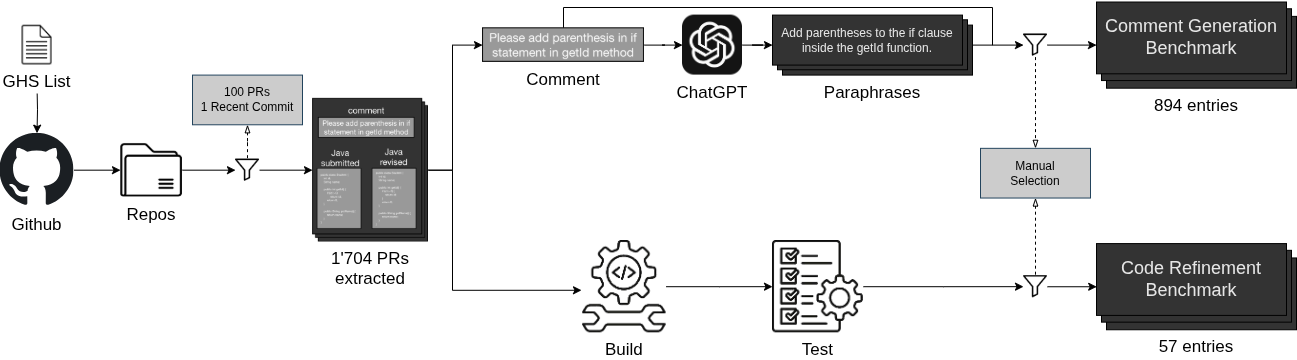
\includegraphics[width=\textwidth]{overview.png}
	\caption{Overview of the data construction pipeline.}
	\label{fig:overview}
\end{figure}

Figure~\ref{fig:overview} illustrates the high-level structure of our dataset construction pipeline.
Starting from a filtered list of GitHub repositories, we extracted 1'704 pull requests containing
exactly one review comment (with optional reply from the author of the PR) and a corresponding code
revision. Each comment was paraphrased using ChatGPT to generate diverse phrasings, yielding 894
entries for the comment generation benchmark. A subset of these (57 entries) also passed all build,
test, and coverage checks, making them eligible for the code refinement benchmark. These refinement
candidates were manually curated to isolate only the changes relevant to the review comment. This
diagram complements the following sections by providing a concrete snapshot of the data flow and
benchmark construction process.

A key design decision is that every included \revComment must explicitly suggest a meaningful
modification to the code. As a result, all triplets are valid instances for the comment generation
benchmark. The code refinement benchmark is built as a strict subset of this data: it only includes
triplets where the \revCode implements the suggestion in the \revComment. Since the refinement task
depends on compiling, testing, and verifying coverage, we limit it to triplets where the comment
refers to a Java file. However, this restriction does not apply to the comment generation benchmark.
To reflect the diversity of real pull requests, we accept any triplet where the comment is
actionable, regardless of the file type involved.

We focused on Java projects and aimed for high quality over quantity. That means we only kept
examples that are self-contained, testable, and likely to be meaningful. As a starting point, we
used the \textit{GHS} dataset and tool introduced by Dabić \etal~\cite{Dabic:msr2021data}, which
supports project sampling for Mining Software Repositories (MSR) studies by providing rich metadata
for over 700'000 GitHub repositories. Their platform made it possible to filter for Java
repositories with relevant properties like number of commits, license, and recent activity.

This section explains how we constructed the dataset, how we defined the two benchmark tasks
(comment generation and code refinement), and how we filtered and validated the data to ensure it’s
useful for evaluating future models.


\subsection{Data Source}

\subsubsection{Repository Sampling}

We began by querying the \textit{GHS} dataset~\cite{Dabic:msr2021data}, a large-scale repository
mining platform that indexes metadata for over 700'000 GitHub projects. Using the web
interface\footnote{\url{https://seart-ghs.si.usi.ch}} we applied two simple filters:

\begin{itemize}
	\item The repository must have had at least 100 pull requests.
	\item The date of the last commit must fall within the year 2025.
\end{itemize}

These criteria ensured that we targeted active, collaborative projects likely to have meaningful
code review activity. We exported the matching repository list in CSV format and used it as input
for our processing pipeline.

We applied minimal filtering beyond that. A small number of repositories were manually excluded
during processing, mostly due to extreme build times or authentication issues.

\subsubsection{Pull Request Selection}
\label{sec:pr-selection}

For each selected repository, we searched for pull requests that reflect a clean and minimal review
interaction. Specifically, we looked for PRs that:

\begin{itemize}
	\item Were successfully merged into the main branch.
	\item Contain either one review comment or two, where the second is a reply from the PR author.
\end{itemize}

The goal is to capture cases where a reviewer leaves a single comment and the author either does not
respond in writing, or replies directly within the thread — which we interpret as an acknowledgment
of the feedback. This keeps the setup simple and avoids ambiguous review discussions.

We made this design choice because we realized early on that it would be difficult to create clean
triplets from pull requests with multiple comments. While we can always locate where each comment
appears in the code, it's much harder to untangle which subsequent code changes correspond to which
comment in an automatic way. This makes it challenging to extract multiple, independent \subCode,
\revComment and \revCode triplets from a single pull request. By focusing on PRs with only one
comment (plus an optional reply), we ensure that each PR maps to a single, self-contained instance.
This keeps the data interpretable and makes the benchmark more reliable.

Of course, even in these single-comment PRs, not all follow-up commits are guaranteed to directly
address the reviewer’s feedback. We handle these exceptions through manual validation, as detailed
later in Section~\ref{sec:manual-selection}.

\subsection{Automated Extraction Pipeline}
\label{sec:pipeline}
Transforming raw pull requests into usable training examples requires more than just scraping
metadata from GitHub. It involves carefully extracting code changes, associating them with reviewer
comments, validating their build and testability, and preserving the relevant context along the way.
To achieve this at scale and with high fidelity, we developed a robust, modular, and fully automated
pipeline. This system processes each pull request independently, performing all necessary
extraction, validation, and archival steps in a reproducible and fault-tolerant manner.

The following sections describe the guiding principles behind the pipeline, its overall
architecture, the key stages involved, and the mechanisms used for error handling and parallel
execution.

\subsubsection{Purpose and Design Philosophy}

The goal of the automated extraction pipeline is to transform raw pull requests from open-source
repositories into structured, high-quality dataset entries suitable for evaluation. To do this
effectively, the system must perform a complex sequence of steps, ranging from low-level repository
operations to high-level semantic filtering, while maintaining reliability, traceability, and
consistency at scale.

This pipeline is designed to be fully automated. Given a set of candidate repositories, it processes
each pull request independently from end to end, requiring no human intervention during execution.
This level of automation is critical for large-scale dataset construction, but it comes with
challenges: repositories vary widely in structure, quality, and tooling, and small inconsistencies
can derail processing unless handled robustly.

To address this, the pipeline is built with three guiding principles:
\begin{enumerate}
	\item \textbf{Isolation and Reproducibility.} All build and test steps are executed inside
	      Docker containers, ensuring that the results are not affected by the host system and can
	      be reproduced reliably.

	\item \textbf{Resilience to Failure.} Each processing step is isolated and allowed to fail
	      independently. A failure in one phase, such as test execution or coverage extraction, does
	      not invalidate the rest of the data. Instead, failures are captured and logged with
	      structured metadata so that partial but useful entries can still be retained.

	\item \textbf{Transparency and Debuggability.} Every step records its outcome and, in the case
	      of failure, the exact reason. This enables downstream analysis of failure rates and causes,
	      and facilitates future improvements to the pipeline itself.
\end{enumerate}

The result is a system capable of ingesting a wide variety of pull requests, gracefully handling
both clean and noisy cases, and producing a structured dataset where each entry includes not only
the final output but also a trace of what succeeded or failed during processing.

\subsubsection{High-Level Architecture}

The pipeline is structured as a sequential series of processing stages, each responsible for a
well-defined operation on a single pull request. These stages are executed one after the other, and
at each step, relevant metadata is recorded and potential errors are caught and stored. This design
promotes clarity, modularity, and traceability throughout the entire process.

At a high level, the pipeline begins by cloning the repository and extracting the relevant code and
comment information from the pull request. It then checks out the code states at the beginning and
end of the pull request, archives these snapshots, and determines whether the comment pertains to
code. If so, the pipeline continues by identifying the build system, attempting to compile the
project, executing the test suite, and extracting coverage metrics. Regardless of success or failure
in any step, a dataset entry is created and tagged with its processing outcome.

Although each pull request is treated independently from a logical standpoint, in practice, the
underlying repository state is shared on disk. For reasons of disk space efficiency, we do not
duplicate the repository for each pull request. As a result, pull requests from the same repository
are processed sequentially to avoid race conditions and state conflicts. However, because
repositories themselves are fully independent, the pipeline is parallelized at the repository level:
different repositories can be processed concurrently without interference. This strategy balances
isolation with scalability, allowing the system to make efficient use of compute resources while
maintaining correctness.

Figure~\ref{fig:pipeline} presents a simplified overview of the pipeline’s control flow. The diagram
groups the processing steps into three main phases: \textit{Setup}, \textit{Build \& Validation
	Assessment}, and \textit{Finalization}. There is also a decision point between \textit{Setup} and
\textit{Build \& Validation Assessment}, \textit{Eligibility Check}, that short-circuits unnecessary
work when the comment is not related to code.

\begin{itemize}
	\item \textbf{Setup}: This phase includes cloning the repository, extracting the diffs and
	      modified files, capturing the review comment, and archiving the relevant commits to preserve
	      a reproducible view of the pull request before and after the review.

	\item \textbf{Eligibility Check}: Before performing more expensive operations, the pipeline
	      checks whether the comment targets a Java source file. This distinction is important because
	      test and build validation are only required for the code refinement task. If the comment
	      does not refer to a Java file, the pipeline skips the build phase entirely and proceeds
	      directly to finalization. These entries are still included in the comment generation
	      dataset, since the task only requires that the \revComment suggests a meaningful change,
	      regardless of the file type involved.

	\item \textbf{Build \& Test Assessment}: For code-related comments, the pipeline identifies the build system,
	      attempts to compile the code, runs the test suite, and tries to generate code coverage using
	      JaCoCo. These steps are executed inside Docker containers for reproducibility.

	\item \textbf{Finalization}: Regardless of success or failure in the previous phases, the
	      pipeline saves the dataset entry along with rich metadata describing the processing outcome,
	      including reasons for failure when applicable.
\end{itemize}

This structure ensures a clean separation of concerns while maintaining extensibility and fault
tolerance. New capabilities or heuristics can be integrated into any phase with minimal disruption
to the rest of the system. The modular layout also enables robust error handling, allowing the
pipeline to continue processing even when individual pull requests encounter issues. This makes the
system scalable and resilient when applied to large and diverse sets of repositories.

\begin{figure}[!htbp]
	\centering
	\begin{tikzpicture}[
			node distance=1cm and 1cm,
			every node/.style={font=\small},
			startstop/.style={circle, draw, minimum size=1cm},
			process/.style={rectangle, draw, rounded corners, minimum width=4cm},
			decision/.style={diamond, draw, minimum width = 4cm, aspect = 2, align=center},
			arrow/.style={->, thick}
		]

		\node (start) [startstop] {Start};
		\node (prep) [process, below of=start, yshift=-.1cm] {Setup};
		\node (iscode) [decision, below of=prep, yshift=-.6cm] {Is comment\\code-related?};
		\node (validation) [process, right of=iscode, xshift=7cm] {Build \& Validation Assessment};
		\coordinate (mid) at ($ (iscode)!0.5!(validation) $);
		\node (save) [process] at ($(mid |- validation.south)+(0,-1cm)$) {Finalization};
		\node (end) [startstop, below of = save] {End};

		% arrows - linear path
		\draw[arrow] (start) -- (prep);
		\draw[arrow] (prep) -- (iscode);
		\draw[arrow] (iscode) -- node [above] {yes} (validation) ;
		\draw[arrow] (iscode) |- node [left] {no}(save) ;
		\draw[arrow] (validation) |- (save);
		\draw[arrow] (save) -- (end);
	\end{tikzpicture}
	\caption{Automated pipeline for processing a single pull request.}
	\label{fig:pipeline}
\end{figure}

\subsubsection{Key Pipeline Stages}

This section provides a more detailed walkthrough of the core stages outlined in
Figure~\ref{fig:pipeline}. Each pull request passes through the same structured sequence of
operations, with intermediate state and outcomes logged to facilitate inspection, debugging, and
dataset filtering.

\paragraph{Setup.} The pipeline begins by cloning the target repository, unless it already exists
locally. To avoid unnecessary downloads and to support resuming interrupted runs, previously cloned
repositories are reused. Once the repository is available, the system retrieves both the base and
merged commits of the pull request. These two commits serve as reference points to extract the code
diffs before and after the review comment.

The system then attempts to extract the content of all files modified by the pull request. This is
done using the GitHub API when possible, and directly from disk as a fallback when the API is
incomplete or fails to deliver consistent results. Special care is taken to record both the pre- and
post-merge versions of each file, as well as to ensure coverage data can be attached to the correct
source snapshot.

Review comments are extracted and filtered to retain only those that reference a specific file and
line range. This is necessary because GitHub occasionally serves comments without reliable line
anchoring. Comments without a valid line mapping are discarded early
in the process to reduce ambiguity downstream.

Both the base and merged states of the repository are archived in compressed form. These serve
distinct purposes. The base state (representing the code before any changes introduced by the pull
request) is primarily stored to provide broader context to models that may benefit from
access to the entire project structure. While the dataset already includes the full content of the
specific files involved in the pull request, some models may require a more holistic view of the
repository to make informed predictions. The merged state, on the other hand, is preserved for
evaluation purposes. In particular, it is used to test model-generated submissions in the context of
the code refinement task. Details of this evaluation setup are discussed further in
Section~\ref{sec:refinement}.

\paragraph{Eligibility Check.} Once the setup phase is complete, the system performs a quick check
to determine whether the review comment is attached to a source code file. If the comment points to
a non-code file (e.g. documentation, configuration files, or assets) it is extremely unlikely that
the suggested change involves actual code behavior. In such cases, running the full build phase,
that includes build, test, and coverage analysis, would be unnecessary and wasteful. To conserve
computational resources and reduce processing time, the pipeline bypasses that phase entirely for
these entries and moves directly to finalization. This early filtering mechanism ensures that only
potentially meaningful code-related changes undergo the more expensive analysis.

\paragraph{Build \& Test Assessment.} For comments that do target Java files, the pipeline enters
the build and test assessment phase. It first detects whether the repository uses Maven or Gradle by
inspecting known build configuration files. This allows it to spin up the appropriate Docker
container, preconfigured with the necessary environment for building and testing Java code.

Once inside the container, the pipeline attempts to compile the codebase. If the build succeeds, it
proceeds to run the test suite. If tests are detected and executed successfully, the system then
attempts to extract code coverage information using JaCoCo. If the project already includes JaCoCo
in its configuration, the system leverages that setup directly. Otherwise, it attempts to inject the
required configuration into the build process. While this injection is not guaranteed to succeed in
all cases, it enables coverage reporting in many repositories that would otherwise lack it.

After coverage reports are generated, the system analyzes them to determine whether the file
affected by the review comment is included in the results. This is done by extracting the fully
qualified class name from the file and searching for it in the coverage data. Due to the presence of
multi-module repositories and inconsistent directory structures, this association is not always
perfect. As discussed in Section~\ref{sec:multi-project-repo}, users must sometimes manually verify
that the reported coverage corresponds to the correct subproject.

\paragraph{Finalization.} At the end of the pipeline, the system records the outcome of each
processing step, including whether the pull request built and tested successfully, whether the
commented file was covered by tests, and whether the comment was code-related. If any step failed,
the reason is logged in structured metadata using a dedicated exception hierarchy. This allows for
filtering and debugging later on.

Every processed pull request results in a dataset entry, even if a phase failed. This is a
deliberate design choice: entries that fail the build phase may still contain useful review comments
for tasks such as comment generation. By capturing the full trace of each pull request—including
what succeeded, what failed, and why—the pipeline produces a dataset that is not only rich in
content but also transparent and debuggable.

\subsubsection{Failure Handling and Debuggability}

One of the key challenges in building a dataset from real-world repositories is handling the wide
range of inconsistencies, misconfigurations, and unexpected edge cases that arise in practice.
Repositories may have incomplete histories, broken builds, missing dependencies, or improperly
formatted comments. Rather than treat these cases as exceptions to be discarded, the pipeline is
designed to process them as first-class outcomes and record their failure modes explicitly.

Each stage of the pipeline is wrapped in fine-grained error handling logic. When a step fails
(whether due to a Git error, an unresolvable build issue, or malformed metadata) the failure is
caught, and a dedicated custom exception class is raised. These exceptions are structured,
categorized, and logged in the metadata of the corresponding dataset entry. This approach allows
each pull request to contribute useful diagnostic information, even when it does not yield a fully
valid instance.

This design serves two purposes. First, it enables comprehensive statistics about failure rates and
patterns across repositories. For example, one can measure how many entries fail at the build step,
how many fail due to missing line mappings in comments, or how often coverage extraction fails due
to JaCoCo injection issues. These insights help guide improvements to the pipeline and provide a
realistic picture of what can be expected when operating at scale.

Second, by retaining partially processed entries and clearly tagging them with their failure
context, the pipeline supports debugging, validation, and experimentation without requiring
re-processing from scratch. Entries that fail the build phase may still contain valuable
content for the comment generation task.

This robust failure management strategy ensures that the pipeline remains resilient in the face of
the inconsistencies inherent to open-source codebases. It allows for high-throughput processing
without sacrificing visibility into what went wrong, and it provides a mechanism for iterative
refinement over time.

\subsubsection{Parallelism and Scalability}

To process a large number of repositories efficiently, the pipeline is designed with parallel
execution capabilities. However, parallelism is applied at the repository level rather than the pull
request level. This distinction is critical due to the way repositories are managed on disk.

During processing, the build, test, and coverage phases operate directly on a local clone of the
repository. Creating separate copies of the repository for each pull request would incur a
substantial disk overhead, especially for large projects. To avoid this, the pipeline reuses a
single local clone per repository. This means that only one pull request per repository can be
processed at a time, ensuring consistency and preventing conflicts caused by concurrent checkouts or
file modifications.

To scale across repositories, the pipeline uses a multi-process architecture where multiple worker
processes handle different repositories in parallel. Each worker runs its own isolated pipeline
instance, with no shared state, and processes one repository at a time. This approach makes full use
of available compute resources while preserving correctness and reproducibility.

Parallelism also helps avoid bottlenecks caused by unbalanced workloads. Some repositories contain
only a handful of pull requests and can be processed quickly, while others (especially those with
extensive histories and complex build steps) take significantly longer. By distributing work across
multiple repositories concurrently, the system avoids having to wait on the slowest task to proceed.

However, true scalability is limited by another important factor: GitHub’s API rate limits. These
constraints, and how the pipeline addresses them, are discussed in the next section.

\subsubsection{Dealing with API Limits and Caching}

A critical bottleneck in any large-scale GitHub data processing pipeline is the platform's API rate
limit. GitHub imposes a cap of 5000 requests per hour per authenticated user. At first glance, this
may appear generous, but in practice, it is quickly exhausted due to how the GitHub Python client
operates.

The library adopts a lazy-loading design: most objects returned from the API are incomplete by
default and only fetch their full data when specific attributes are accessed. While this is
efficient for bandwidth and memory usage, it results in many additional network calls during regular
use. A single pull request may require dozens requests to fetch metadata, commit histories,
comments and file contents.

Fortunately, the library provides automatic handling of rate limit exhaustion. When the limit is
reached, it enters a waiting state and resumes once requests become available again. This makes it
safe to run the pipeline with multiple threads or processes: each one will automatically pause and
continue as needed without crashing or violating GitHub’s usage policies.

Despite this robustness, long pauses can be impractical when running large-scale crawls. To mitigate
this, the pipeline includes two layers of caching:

\begin{itemize}
	\item \textbf{HTTP-level caching:} The GitHub responses themselves are cached locally using an
	      auxiliary Python library, allowing the pipeline to skip API calls for data that has already
	      been retrieved. This not only saves bandwidth and time but also avoids rate limits entirely
	      for cached objects.

	\item \textbf{Pipeline-level checkpointing:} The system tracks which pull requests have already
	      been processed. If the pipeline is interrupted or restarted, it can pick up where it left
	      off without reprocessing completed work. This enables stop-and-resume operation, which is
	      especially valuable for long runs or incremental dataset builds.
\end{itemize}

While the GitHub Python library lacks thorough documentation, its internal behavior, once inspected,
proves reliable and well-suited for automation at scale. On several occasions, the implementation
had to be understood by directly reading its source code. Nonetheless, once these behaviors are
accounted for, the client operates smoothly, and the pipeline is able to run unattended for extended
periods, managing its own retries and pacing.

These design decisions—automated rate limit handling, layered caching, and task
checkpointing—combine to make the pipeline not just scalable in theory, but practically usable for
large-scale, real-world dataset construction.

\subsection{Build, Test \& Coverage}


\subsubsection{Motivation and Purpose}

Ensuring that each pull request can be built, tested, and instrumented for coverage is a key step in
constructing a dataset that goes beyond static code analysis. This phase is not just a validation
step for technical completeness, it also lays the groundwork for more robust evaluation. The ability
to compile and execute the code opens up the possibility of behavior-based assessment, which is
critical when evaluating code refinement models.

In contrast to similarity-based metrics such as CodeBLEU, which penalize variations in syntax even
when semantics are preserved, test-based evaluation allows for multiple valid implementations to be
accepted as long as they do not introduce regressions. While passing tests do not guarantee the
correctness of a change, they do strongly suggest that the change is not invalid. Failing tests, on
the other hand, clearly indicate broken behavior. This framing enables more realistic and flexible
model evaluation, better aligned with real-world development practices.

\subsubsection{Test Detection}

The first step is to determine whether the repository contains any form of automated
testing. This is accomplished by scanning the build configuration files for known testing libraries
(e.g., JUnit, TestNG, Mockito) and build system keywords such as \path{testImplementation} or
\path{functionalTests}. In addition to static analysis of the build file, the system also
inspects conventional test directories, such as \path{src/test/java} or \path{test/}, which
frequently contain unit or integration tests. This dual approach increases the reliability of test
detection across a broad set of repository structures.

\subsubsection{Execution Environment}
\label{sec:exec-env}

To ensure reproducibility, consistency, and isolation from the host system, all compilation and test
operations are executed within Docker containers. Two container environments are maintained,
corresponding to the two supported Java build systems: Maven and Gradle. Each container includes the
necessary tools, dependencies, and environment settings to execute a typical Java project. This
ensures that the results are not affected by host-specific variations, such as Java versions, OS
configuration, or missing libraries.

The architecture is designed with extensibility in mind. Build system support is modularized so that
new systems (such as Ant or Bazel) can be integrated by adding new handler classes and corresponding
container definitions. This separation of concerns facilitates future expansion to accommodate more
diverse types of software projects. Moreover, because the interface between the build system logic
and the rest of the pipeline is language agnostic, it is hypothetically straightforward to extend
support beyond Java and handle projects written in entirely different programming languages,
provided suitable build and test tooling exists for them.

\subsubsection{Coverage Generation}

Once a repository has been successfully built and tested, the next objective is to collect code
coverage data. This is primarily done using JaCoCo, a widely adopted tool for Java coverage
reporting. If the project is already configured with JaCoCo, the system attempts to run its existing
configuration directly. If this fails, typically due to the absence of the plugin, the system attempts
to inject JaCoCo manually into the build file, modifying the configuration to include the required
setup for coverage generation.

Care is taken to preserve the integrity of the build system: the original configuration is backed up
and restored if the injection fails. When successful, the injected configuration allows for the
generation of XML coverage reports, which are then parsed to extract coverage percentages for
individual files.

\subsubsection{Handling Multi-Project Repositories}

\label{sec:multi-project-repo}
A major challenge arises when dealing with large repositories that are organized into multiple
subprojects. These may be loosely coupled, deeply nested, or follow custom directory conventions.
Because of this structural diversity, it is difficult to reliably map a given Java file to a
specific coverage report. To approximate this mapping, the system extracts the fully qualified class
name of each commented file and searches for it across all available coverage files. If found, the
file is marked as covered.

This approach, while pragmatic, is not foolproof. It does not guarantee that the coverage report
belongs to the same subproject as the file in question. Given the variability in repository layout,
automatic resolution of this ambiguity is not feasible. Users are therefore advised to manually
verify coverage associations in cases where accuracy is critical.

\subsubsection{Enabling Flexible Evaluation}

By ensuring that the code in each pull request is buildable and testable, the dataset allows for a
richer model evaluation framework. Unlike static metrics that enforce a rigid similarity standard,
test-based validation supports functional correctness. This means that a model can propose diverse
implementations in response to reviewer comments, as long as the resulting code passes all tests. In
effect, this introduces a behavior-first evaluation protocol that aligns more closely with how
developers themselves judge correctness: not by form, but by function.

In summary, this phase adds significant value to the dataset by grounding it in real, executable
code, and by enabling flexible, semantically meaningful evaluation. Despite the technical challenges
involved—such as inconsistent configurations, incomplete test setups, and structural complexity—this
approach provides a much more powerful basis for training and evaluating automated code refinement
systems.

\subsection{Manual Selection}
\label{sec:manual-selection}

While the construction of the dataset is driven by automation to ensure scale and consistency, there
remain several aspects that fundamentally depend on human judgment. One of the most important among
these is the annotation of intent and follow-through: determining whether a reviewer’s comment
suggests a change, and whether that change was subsequently implemented in the pull request.

\subsubsection{Comment Classification}
The first layer of this process involves evaluating the nature of the review comment itself. Not all
comments are meant to trigger code modifications. Many comments are purely informational, offering
optional improvements or clarifications that do not warrant actual changes. Some comments are not
directly related to the current pull request but are instead left as notes for future work. These
typically refer to changes that should be made after the branch has been merged with another one,
but which cannot be carried out within the scope of the current pull request due to technical
constraints. Others might highlight a section of code without proposing any specific action. In
order to ensure that the dataset captures meaningful reviewer-author interactions, it is necessary
to distinguish between comments that suggest actionable modifications and those that do not.

A particularly nuanced category of comments consists of those framed as questions. While at first
glance they may appear less directive than imperative statements, questions often carry implicit
suggestions. These can be roughly divided into two main types. The first are rhetorical questions,
which are generally straightforward to interpret. These tend to imply strong disapproval or an
obvious recommendation, masked in the form of a question. For example, a reviewer might write,
\textit{``Can you move this declaration down closer to where it's used?''} or \textit{``Isn't this
	redundant with the previous check?''} In most cases, the intent behind such comments is clear: they
point out something that should be removed, refactored, or reconsidered.

The second type of question-based comment is more difficult to classify. These are genuine
inquiries, often posed in good faith, reflecting uncertainty or opening a discussion. They may
express doubt about a design choice, inquire about alternative implementations, or question whether
a particular solution addresses the intended problem. For instance, a reviewer might ask,
\textit{“Would it make sense to use a stream here instead of a loop?”} or \textit{“What happens if
	this input is null?”} The challenge with these types of comments is that they can be interpreted in
multiple ways. Some reviewers may expect an immediate change, while others are simply requesting
clarification. In many cases, the boundary between suggestion and inquiry is blurry, and
classification depends on context: including the tone of the comment, the review history, and even
the norms of the repository or organization. As a result, the decision to treat such a comment as a
change suggestion often comes down to the judgment of the person performing the manual annotation.

\subsubsection{Assessing Implementation of the Change}
Once a comment is identified as suggesting a change, the next step is to verify whether the change
was actually implemented. This involves inspecting the commits made after the comment was posted and
analyzing the diffs introduced. However, this is not as straightforward as it may seem. In modern
development workflows, especially those influenced by continuous integration and continuous
deployment (CI/CD) practices, it is common for the pull request branch to be updated with changes
from another branch, such as \texttt{main} or \texttt{dev}, before it is merged. This is often done
to resolve merge conflicts, bring in recent bug fixes, or ensure compatibility with the latest
version of the codebase. While such merges are necessary from an engineering perspective, they
introduce significant noise from the point of view of dataset construction.

When another branch is merged into the pull request, it can bring in a large number of changes that
are unrelated to the comment or even to the pull request itself. As a result, the diffs that appear
after the comment may include modifications that are completely irrelevant to the interaction being
studied. This creates a challenge: how can we isolate the changes that were made in response to the
comment from the rest?


\subsubsection{Selective Diff Curation}

To address this issue, the system incorporates a manual selection step where the user is shown the
diffs produced after the comment and is asked to select which hunks (blocks of code changes) are
relevant to the comment. This allows for precise filtering of the changes and helps construct a
cleaner, more focused dataset where only the diffs that represent a response to the review comment
are preserved.

In some cases, the situation is further complicated by the proximity of changes. Even when
irrelevant changes originate from merges or unrelated commits, they may occur in the same file or
even in adjacent lines to the relevant ones. This results in hunks that contain both the actual
response to the comment and unrelated code. Because the standard diff format groups nearby changes
into a single hunk, it becomes impossible to separate them without manual intervention. To deal with
such situations, the system provides the ability to edit the hunks directly. Users can manually trim
the diff to retain only the portions that directly address the reviewer’s feedback, discarding the
unrelated ones. This kind of fine-grained control is essential for preserving the integrity and
specificity of the dataset.

By performing this dual-level manual selection — first identifying whether a comment suggests a
change, and then isolating the relevant diff hunks — the dataset maintains a high degree of
fidelity. It captures meaningful reviewer-author interactions and filters out unrelated noise
introduced by collaborative development practices. This ensures that the final data is not only
accurate but also truly representative of how developers respond to feedback during the code review
process.

\subsubsection{Manual Selection as a Design Choice}

The decision to include a manual selection step was not an afterthought, but a deliberate design
choice. Prior work has shown that fully automated dataset construction methods often introduce a
significant amount of noise—whether due to misclassified comments, ambiguous code changes, or
incidental modifications unrelated to reviewer feedback. Rather than aiming for scale at the expense
of quality, we chose to prioritize precision and relevance. By hand-picking the instances we deemed
meaningful and representative, we ensured that the dataset would reflect true reviewer-author
interactions, with clearly identifiable suggestions and corresponding responses. This curated
approach allows for more reliable evaluation of models in tasks that require nuanced understanding
of code review dynamics.

\subsection{Paraphrase Generation}
\label{sec:paraphrases}

One of the key contributions of this work is the introduction of paraphrases into the dataset, which
addresses a major limitation in existing benchmarks. Most prior work in this space evaluates model
output using exact or near-exact string matching metrics such as BLEU or ROUGE. However, these
metrics are highly sensitive to surface-level variations and fail to account for semantically
equivalent outputs that differ in length or wording.

For instance, consider the following real-world example from the work of Tufano \etal
\cite{tufano:icse2022}. A reviewer commented:

\begin{quote}
	\textit{“Please make this one a variable as well.”}
\end{quote}

In response, a model predicted the following output:

\begin{quote}
	\textit{“Extract the building of the ResponseMessage to its own variable (in eclipse, select the
		text, right-click > refactor > extract local variable / select code + shift + alt + L). This
		will make the code a bit more readable, especially when you’ll be passing in other things besides
		the ResponseMessage.”}
\end{quote}

While both comments clearly convey the same request, they differ substantially in structure,
phrasing, and length. As a result, surface-level comparison metrics like BLEU score assign an
unjustifiably low similarity score, even though the semantic equivalence is clear to a human
reviewer.

To mitigate this issue, we introduce a set of paraphrases for each reviewer comment in the dataset.
These paraphrases are generated using a large language model (specifically, the \texttt{o4-mini}
variant of ChatGPT) guided by a carefully designed prompt. The prompt instructs the model to
generate up to ten paraphrases that preserve the original meaning exactly, while varying in
verbosity and structure.

The prompt used is as follows:

\begin{quote}\ttfamily
	You will be given a code change ("Code change") and a code review comment ("Reviewer comment")
	from a reviewer who reviewed the code.\\
	Generate as many non-trivial and meaningful paraphrases as possible (maximum 10) for the
	reviewer's comment.\\
	The comment refers to the part of the code identified by the special tag
	\texttt{<commented\_line>}.\\
	Each paraphrase should differ in length: include some extremely concise version of the comment,
	some highly verbose version, and some that are roughly the same length—while always preserving
	the original meaning exactly.\\
	\\
	Generate the paraphrase (and nothing else) in the following format:\\
	\\
	Paraphrase\#1: \textless comment\_paraphrase\textgreater\\
	Paraphrase\#2: \textless comment\_paraphrase\textgreater\\
	\ldots\\
	Paraphrase\#10: \textless comment\_paraphrase\textgreater\\
	\\
	"Code change"\\
	\textless code\_change\textgreater\\
	\\
	"Reviewer comment"\\
	\textless reviewer\_comment\textgreater
\end{quote}

This setup ensures a diversity of phrasing that can better reflect the natural variability in human
feedback. The generated paraphrases are manually reviewed to ensure they faithfully preserve the
semantic content of the original comment.

These paraphrases make it possible to compute similarity metrics, such as BLEU, against a richer set
of reference outputs. This, in turn, provides a more accurate and tolerant evaluation of model
predictions. Details on how paraphrases are used in the benchmark evaluation are provided in
Section~\ref{sec:paraphrases-check}.

\subsection{Dataset Schema \& Serialization}

The dataset is designed to be both expressive and flexible. Each entry represents a single pull
request and contains a rich set of data capturing the code, the reviewer comments, the surrounding
context, and the repository’s response.

\subsubsection{Schema Overview}

Each entry in the dataset encapsulates multiple layers of information. At the core is the
\texttt{metadata} object, which includes identifying fields such as repository name, pull request
number, and commit hashes. It also contains metadata about the PR’s outcome, such as whether the
project built successfully, whether the file under review was covered by tests, and whether the
comment was judged to suggest a change.

The entry also stores:
\begin{itemize}
	\item The full set of \texttt{comments}, including body text, line ranges, and paraphrases.
	\item The \texttt{files} affected by the pull request, each annotated with its content before
	      and after the change, test coverage metrics, and whether it is code-related.
	\item Two sets of \texttt{diffs}: those between the opening of the PR and the reviewer comment
	      (``before''), and those occurring after the comment (``after'').
\end{itemize}

Together, these components allow for rich modeling of code review interactions over time.
Specialized views of this data, used for comment generation or code refinement tasks, can be derived
through structured filtering.

\subsubsection{Design Rationale}

The schema is built around the principle of modularity. Rather than entangling comment logic, diff
parsing, and code coverage into a flat structure, each concept is separated into its own dedicated
field or object. This makes it easy to reason about and operate on specific parts of the dataset
independently, for example, isolating all comments that suggest a change, or extracting only the
diffs related to code files.

\subsubsection{Serialization Formats}

The dataset supports several serialization modes, depending on the intended downstream task. These
include:
\begin{itemize}
	\item \texttt{full}: All fields are retained, giving a complete view of each entry.
	\item \texttt{comment\_gen}: Only includes entries where the reviewer comment suggests a change,
	      and retains just the code state and diffs before the comment. Useful to give as input to
	      a model for the comment generation task.
	\item \texttt{code\_refinement}: Filters to entries where the change was both suggested,
	      implemented and covered by tests. Includes the comment and the ``before'' diff, but omits
	      unrelated fields. Useful to give as input to a model for the code refinement task.
	\item \texttt{webapp}: A lightweight format that includes only metadata and comments, intended
	      for use in the webapp, so that it doesn't take long to load in memory.
\end{itemize}

Each mode produces a JSON file that is readable, compact, and suitable for different types of
experiments or tools. In addition, the serialization process allows for filtering out entries that
do not meet the criteria for inclusion in the dataset, such as comments that do not suggest a change
or pull requests that failed somewhere along the pipeline described in Section \ref{sec:pipeline}.
These “faulty” entries are not part of the intended dataset and are retained only as a form of
internal logging. They serve two main purposes: enabling detailed analysis of failure patterns
(e.g., identifying how many entries failed due to missing tests or broken builds), and helping
future efforts to improve the pipeline itself. The dataset, as serialized for
evaluation, is meant to consist exclusively of clean, validated entries that support the task of
comment generation or refinement.

\subsubsection{Use Case-Driven Filtering}

This flexibility allows researchers and engineers to tailor the dataset to the task at hand. For
example, a model trained to generate review comments may only require the pre-comment diff and
associated files. A refinement model, on the other hand, benefits from both the comment and the
changes made after it, with accurate annotation of whether the diff actually addressed the
suggestion.

The ability to serialize the dataset in multiple views avoids the need to rerun the full pipeline
every time a new task is proposed. It also supports experimentation and benchmarking across
different problem formulations while keeping the core data consistent.

\subsubsection{Extensibility and Programmatic Access}

Beyond serialization, the dataset class includes convenience methods for loading, filtering, and
mapping entries by ID. Internally, the logic is implemented in a way that is agnostic to language or
repository structure. This makes it easy to adapt the system to future extensions, such as
supporting other programming languages or integrating with other evaluation pipelines.

Overall, the dataset schema and its serialization logic reflect a balance between structure,
flexibility, and practical usability, ensuring that the data can evolve alongside the research it
supports.

\subsection{Phases of Dataset Curation}

The dataset construction process was performed in two phases, each with distinct strategies for
repository filtering and pull request validation.

\subsubsection{Initial Filtering and Manual Validation}

The first phase began with a list of 4'795 repositories sourced from the GHS dataset. To narrow the
scope, a pre-filtering step was applied. Each repository was cloned, and the following conditions
were checked on the most recent commit of the default branch:

\begin{itemize}
	\item The project uses a supported build system (e.g., Maven or Gradle).
	\item It compiles successfully.
	\item All tests pass.
	\item At least one test is present.
\end{itemize}

Only repositories satisfying all criteria were retained, reducing the list to 398 projects. From
these, all available PRs were extracted, yielding 1'681 PRs in total. After manually validating
whether the comments suggested changes and whether those changes were implemented, a set of 985 PRs
was finalized for the comment generation task.

A significant limitation emerged at this stage: although 22 PRs were both compilable and testable,
none of them met the required test coverage conditions. This rendered the initial dataset
insufficient for the code refinement task.

\subsubsection{Updated Construction and Expanded Dataset}

In response, the second phase re-ran the dataset construction on the full set of 4'795 repositories.
This iteration incorporated improvements to the data collection pipeline, specifically:

\begin{itemize}
	\item Coverage checks were moved to the construction stage, rather than being deferred to manual
	      filtering.
	\item A stricter coverage criterion was applied: the PR must have at least one coverage file
	      associated with the commented file, and all reported files must exhibit non-zero line
	      coverage.
\end{itemize}

These changes led to a more refined classification of pull requests valid for code refinement.
Previously, a PR was considered valid if it compiled and tested successfully, regardless of test
coverage. Now, a PR is only considered valid if it is (a) code-related, (b) builds and tests pass,
and (c) the coverage condition is satisfied.

\subsubsection{Observations}

The improvements made between the two runs significantly enhanced the reliability of the dataset
construction process. While the first run provided useful insights, such as the overall rate of PR
failures and the effectiveness of the manual filtering. It primarily served as a proving ground for
iterating on the pipeline. Despite being limited to 398 repositories, it helped validate the
extraction logic and informed adjustments to the coverage evaluation and PR validation mechanisms.

Once the pipeline was considered robust, the second run extended the process to all 4'795
repositories. This larger scope was essential to capture a broader and more diverse set of eligible
PRs, especially for the code refinement task, that depend on accurate coverage information.

Although the updated process improves coverage filtering, many PRs still fail the coverage check.
One possible way to increase the number of PRs eligible for the refinement task would be to manually
write targeted tests for cases where the code compiles and tests pass, but the changed lines are not
yet covered.

\subsection{Dataset Statistics}

This section presents statistics from both phases of dataset construction. We begin by analyzing the
dataset derived from the 398 pre-filtered repositories. This smaller-scale dataset was the only one
subjected to manual selection, given its more manageable size of 1'681 pull requests. It allows us
to examine the failure distribution across PRs and the impact of manual validation on final PR
eligibility.

We then turn to the second dataset, built from the full set of 4'795 repositories. Although no
manual filtering was applied to this version, the insights gained from the first dataset provide a
useful baseline for interpreting its structure and expected failure patterns.

\subsubsection{Initial Dataset: Pre-filtered Repositories}
\label{sec:stat-small}

Before scaling up to a broader corpus, we conducted an initial run of the dataset construction
process on a smaller, pre-filtered set of repositories. Table~\ref{tab:initial-distribution}
summarizes the outcome of this first stage. A substantial portion of the PRs (over 64\%) encountered
issues during automated processing. These ranged from compilation failures to missing commits or
broken diffs. About 27\% of the total were not code-related (i.e., the review comments did not
target source code files). The remaining slices represent entries that passed both build and test
phases, but only 4.87\% were covered by tests.

\begin{table}[ht]
	\centering
	\begin{tabular}{lrr}
		\toprule
		\textbf{Subset}                           & \textbf{Count} & \textbf{Percentage} \\
		\midrule
		Total PRs                                 & 1'704          & 100.00\%            \\
		Had issues during processing              & 1'094          & 64.20\%             \\
		Not code-related                          & 456            & 26.76\%             \\
		Builds and passes tests, not covered      & 71             & 4.17\%              \\
		Builds and passes tests, covered by tests & 83             & 4.87\%              \\
		\bottomrule
	\end{tabular}
	\caption{Breakdown of initial dataset (1'704 PRs)}
	\label{tab:initial-distribution}
\end{table}

To better assess data quality, we manually reviewed the full set of 1'704 entries extracted in the
initial run. Each entry was tagged based on whether the \revComment actually suggested a meaningful
code change. The outcome of this annotation process was a curated subset of 894 entries, containing
only those instances where the comment was determined to be actionable.
Table~\ref{tab:manual-selection-distribution} shows the composition of this manually selected group.
The distribution of processing issues and coverage is broadly similar to the full set, but one
notable difference is a slight increase in the proportion of test-covered PRs, which rises to
7.61\%.

\begin{table}[ht]
	\centering
	\begin{tabular}{lrr}
		\toprule
		\textbf{Subset}                           & \textbf{Count} & \textbf{Percentage} \\
		\midrule
		Selected PRs                              & 894            & 100.00\%            \\
		Had issues during processing              & 506            & 56.60\%             \\
		Not code-related                          & 284            & 31.77\%             \\
		Builds and passes tests, not covered      & 47             & 5.25\%              \\
		Builds and passes tests, covered by tests & 57             & 6.38\%              \\
		\bottomrule
	\end{tabular}
	\caption{Breakdown of manually selected subset (894 PRs)}
	\label{tab:manual-selection-distribution}
\end{table}

It is worth emphasizing that entries which encountered issues during processing are not necessarily
unusable. In particular, if the code state at the beginning of the PR, the diff before the comment,
and the comment itself are all available, the instance remains a valid input for the comment
generation task. While such examples are excluded from the refinement benchmark due to lack of test
feedback, they still represent meaningful reviewer interactions.

This initial run exposed the limitations of automatic extraction and set a realistic baseline for
expected yield: only a small fraction of PRs (roughly 4.81\%) were both testable and covered. We
hoped to see a similar or better outcome in the expanded dataset constructed from a broader
repository set. Unfortunately, as later sections show, this expectation did not hold.

The full processing of this dataset using five parallel threads took roughly 7 hours, thanks to full
caching of GitHub API requests. Without caching, the same run would be subject to API rate limits
and request overhead, and is estimated to require approximately five days to complete.

\paragraph{Failure Analysis}

The initial dataset also provided a valuable overview of the types of failures encountered during
automated processing. Table~\ref{tab:failure-distribution} summarizes the most common failure
categories observed during the extraction pipeline. For readability, only the most frequent issues
are shown explicitly; the remaining cases have been grouped under ``Other issues.''

\begin{table}[ht]
	\centering
	\begin{tabular}{lrr}
		\toprule
		\textbf{Failure Reason}                             & \textbf{Count} & \textbf{Percentage} \\
		\midrule
		Failed to compile                                   & 296            & 21.14\%             \\
		Commented file not in any coverage report           & 153            & 8.98\%              \\
		Failed to test                                      & 120            & 7.04\%              \\
		Comment not associated with a specific file or line & 116            & 6.81\%              \\
		Referenced line absent in pre-comment diffs         & 109            & 6.40\%              \\
		Couldn't get diffs after last commit                & 84             & 4.93\%              \\
		Couldn't fetch PR's merge commit\footnotemark       & 78             & 4.58\%              \\
		Couldn't execute coverage tool (JaCoCo)             & 60             & 3.52\%              \\
		No tests found                                      & 37             & 2.17\%              \\
		Failed to extract test results                      & 14             & 0.82\%              \\
		Other issues                                        & 27             & 1.58\%              \\
		\bottomrule
	\end{tabular}
	\caption{Most common failure reasons in initial dataset (1'704 PRs)}
	\label{tab:failure-distribution}
\end{table}

\footnotetext{This is a known limitation of the GitHub API, as discussed
	in~\cite{stackoverflow-merge-sha}. Although we implemented the workaround suggested in the discussion,
	it only partially mitigated the problem. Some PRs still fail due to missing or inaccessible merge
	commits.}

These failure cases fall into several categories: build issues, coverage limitations, GitHub API
inconsistencies, and project-specific anomalies (e.g., deleted or renamed files, unusual repository
structures). While some of these failures are inherent to the dynamic nature of open-source
projects, others reveal areas where the pipeline could be hardened.

In practice, many of these failure cases were manually inspected during the first dataset run, which
itself was re-executed multiple times as the pipeline was refined. These iterations helped identify
edge cases and improve the robustness of the extraction process. Additional improvements were made
afterward and incorporated into the second dataset run, such as a more thorough coverage check and
multithreading, among others. Nonetheless, a portion of these issues, such as incomplete
coverage reports or unusual file responses, remain difficult to resolve automatically. Targeted
manual investigation or fallback mechanisms could further reduce failure rates and increase the
number of valid PRs in future iterations.

\subsubsection{Expanded Dataset: Full Repository Set}
\label{sec:stat-expanded}

After validating the extraction pipeline on a smaller pre-filtered sample, we extended the dataset
construction to the full set of 4'795 Java repositories sourced from the GHS dataset. Unlike the
initial phase, no pre-filtering was applied to ensure buildability or test presence. This choice
aimed to better understand the pipeline’s behavior under more realistic, large-scale conditions, and
to increase the likelihood of finding a larger number of PRs that compile, test successfully, and
are covered by tests.

The repositories were processed in descending order of stargazers, based on the assumption that
projects with a higher number of stars are likely to be of higher quality. The rationale was that
more prominent projects are generally better maintained and enforce stricter contribution
guidelines, which could lead to cleaner, more meaningful PRs. However, this strategy may have
backfired. Projects with high visibility also tend to be larger, more complex, and more prone to use
custom or non-standard build systems, making them harder to compile and test automatically.

The full run was executed over the course of 10 days using five concurrent threads. During this
time, the system managed to process only about 300 repositories, revealing the hidden cost of
attempting to extract usable data from large-scale, real-world projects.
Table~\ref{tab:expanded-distribution} shows the final breakdown of this expanded dataset. Out of
16'376 processed pull requests, 75.89\% encountered issues during processing. Only 0.32\% passed the
full build and test phase and were covered by tests: just 52 PRs across the entire run. This
highlights a critical bottleneck in relying on automated evaluation, especially in large,
heterogeneous codebases.

\begin{table}[ht]
	\centering
	\begin{tabular}{lrr}
		\toprule
		\textbf{Subset}                           & \textbf{Count} & \textbf{Percentage} \\
		\midrule
		Total PRs                                 & 16'376         & 100.00\%            \\
		Had issues during processing              & 12'428         & 75.89\%             \\
		Not code-related                          & 3'948          & 24.11\%             \\
		Builds and passes tests, not covered      & 29             & 0.18\%              \\
		Builds and passes tests, covered by tests & 52             & 0.32\%              \\
		\bottomrule
	\end{tabular}
	\caption{Breakdown of expanded dataset (16'376 PRs)}
	\label{tab:expanded-distribution}
\end{table}

The low yield of covered entries is partly explained by the nature of the selected repositories. In
particular, 2'714 pull requests (16.65\%) failed because the pipeline could not locate a
recognizable build file. Another 4'612 (28.29\%) failed at the compilation stage. These numbers are
not unexpected, as the repositories were drawn directly from GHS without any guarantee that they
used supported build systems. Given the size and complexity of many of these projects, it's likely
that a significant portion rely on custom build setups that are difficult or impossible to replicate
automatically.

In hindsight, this ordering strategy, based purely on stargazer count, proved suboptimal. Although
it increased the likelihood of encountering high-quality review interactions, it also severely
limited the number of exploitable PRs due to technical constraints. A more effective ordering or
selection heuristic has yet to be discovered.

On the positive side, the high volume of PRs yielded by these large projects provides a rich pool of
potential instances for the comment generation task. While the total number of PRs (16'376) is too
large to manually go through, we hypothesize that the overall quality, once filtered, could be quite
high. This hypothesis remains to be tested through a more targeted validation effort.

Fortunately, the modularity of the pipeline enables future improvements in filtering. One promising
direction is the addition of a lightweight classification step during the setup phase, where a large
language model (either an online service or a locally fine-tuned model) is queried to assess whether
a comment suggests a change. This would allow researchers to pre-filter PRs based on semantic
intent, substantially reducing the manual workload. For instance, the model could be asked:
\textit{``Does this comment request any change or modification to the code?''} This fast and
effective filtering layer would enable downstream manual curation to focus only on PRs likely to
contain meaningful reviewer-author interactions.

In summary, the expanded dataset exposed the practical limits of automated extraction in
uncontrolled environments. While the raw volume of data is promising, a better prioritization
strategy and tooling to assist in manual triage are essential for building high-quality
benchmarks at scale.


\subsubsection{Descriptive Statistics and Distribution Insights}

Beyond basic counts and processing outcomes, this section explores a series of descriptive
statistics that offer a more nuanced view of the dataset’s composition and structure. These
statistics help quantify how the data is distributed across repositories, how verbose the comments
are, and how much code is typically changed before and after the review comments. This analysis also
highlights the impact of manual selection on the relevance and clarity of the diffs retained for
model input.

\paragraph{Distribution of PRs per repository}
The selected dataset, comprising 894 manually curated pull requests, spans a total of 168
repositories. As shown in Figure~\ref{fig:pr-dist}, the distribution of PRs per repository is highly
skewed. A significant number of repositories contribute only a handful of PRs: half of them provide
two or fewer, while a few repositories dominate the dataset with dozens of entries.

\begin{figure}[ht]
	\centering
	\begin{tikzpicture}
		\begin{axis}[
				width=0.85\linewidth,
				height=8cm,
				ybar,
				bar width=5pt,
				xlabel={Number of PRs per Repository},
				ylabel={Number of Repositories},
				grid=major,
				title={Distribution of PR Counts},
				xmin=0,
				enlarge x limits=0.05,
				ymin=0,
				hist={
						bins=30,
						data min=1,
						data max=91
					}
			]
			\addplot+[
				hist
			] table [y index=1] {data/repo2pr.dat};
		\end{axis}
	\end{tikzpicture}
	\caption{Histogram of PR counts per repository, based on the selected dataset of 894 entries
		from 168 repositories. Each bar shows how many repositories contributed a given number of pull
		requests.}
	\label{fig:pr-dist}
\end{figure}



\paragraph{Repository Breakdown by Task.}
As seen in Figure~\ref{fig:pr-dist} not all repositories contribute equally across tasks.
Tables~\ref{tab:top-repos-comment} and~\ref{tab:top-repos-refinement} show the top five repositories
for comment generation and code refinement respectively. For comment generation, a small number of
repositories make up a large portion of the total dataset. For example, \path{magefree/mage} alone
contributes over 10\% of the selected entries. In contrast, the code refinement task draws from a
smaller, more selective subset of PRs, making each contributing repository more prominent.
Interestingly, \path{OpenAPITools/openapi-generator} appears in both lists, reflecting both its
comment activity and the fact that its build and test setup was compatible with the pipeline. This
dual presence suggests that certain projects are particularly well-suited for automated benchmark
extraction.

\begin{table}[ht]
	\centering
	\begin{tabular}{lrr}
		\toprule
		\textbf{Repository}                         & \textbf{PRs} & \textbf{\% of Total} \\
		\midrule
		magefree/mage                               & 91           & 10.18\%              \\
		OpenAPITools/openapi-generator              & 63           & 7.05\%               \\
		blackducksoftware/detect                    & 45           & 5.03\%               \\
		wso2-extensions/identity-inbound-auth-oauth & 31           & 3.47\%               \\
		ome/bioformats                              & 27           & 3.02\%               \\
		\bottomrule
	\end{tabular}
	\caption{Top 5 repositories by number of PRs for the comment generation task (894 total PRs).}
	\label{tab:top-repos-comment}
\end{table}

\begin{table}[ht]
	\centering
	\begin{tabular}{lrr}
		\toprule
		\textbf{Repository}             & \textbf{PRs} & \textbf{\% of Total} \\
		\midrule
		OpenAPITools/openapi-generator  & 10           & 14.71\%              \\
		googleapis/java-spanner         & 6            & 8.82\%               \\
		googleapis/java-storage         & 6            & 8.82\%               \\
		googleapis/java-bigtable        & 5            & 7.35\%               \\
		googleapis/java-bigquerystorage & 4            & 5.88\%               \\
		\bottomrule
	\end{tabular}
	\caption{Top 5 repositories by number of PRs for the code refinement task (68 total PRs).}
	\label{tab:top-repos-refinement}
\end{table}

\paragraph{Tokens per Comment.}
To better understand the variability in reviewer feedback, we examined the number of tokens per
comment. For this analysis, we defined a token as any non-zero-length sequence of contiguous
alphanumeric characters. As shown in Figure~\ref{fig:token-histograms}, most comments are short and
concise: the median is 14 tokens, with the third quartile at 25. A few comments are significantly
longer, reaching up to 935 tokens. These longer entries are mostly produced by automated bots that
perform static analysis and report detailed findings. The presence of both short and long comments
in the dataset is useful, as it provides naturally varied ground truth targets. Since one of the
goals of this benchmark is to support paraphrase generation of different lengths (as discussed in
Section \ref{sec:paraphrases}), having original comments that span a wide range of verbosity is a
strength of the dataset.

\begin{figure}[ht]
	\centering
	\begin{tikzpicture}
		\begin{axis}[
				width=0.85\linewidth,
				height=5cm,
				ybar,
				bar width=3pt,
				xlabel={Tokens per Comment},
				ylabel={Number of Comments},
				grid=major,
				title={Token Count Distribution per Comment},
				ymin=0,
				enlarge x limits=0.05,
			]
			\addplot+[
				hist
			] table [y index=0] {data/tokens2count.dat};
		\end{axis}
	\end{tikzpicture}

	\caption{Histogram of token counts per comment in the selected dataset. Each bar represents the
		number of comments whose token counts fall within a given range, determined by the bin width.}
	\label{fig:token-histograms}
\end{figure}

\paragraph{Size of Diffs and File Scope Before the Comment.}
To characterize the context available prior to each reviewer comment, we examined two key
properties: the total size of the diff and the number of files modified. As shown in
Figure~\ref{fig:diff-before}, the diff sizes vary widely, with a median of 105.5 lines and some pull
requests modifying nearly 2'000 lines of code. The majority of PRs fall below 500 changed lines,
but a long tail of very large changes exists. We also looked at how many files were affected before
the comment. Here, the median is 3 files per PR, with 75\% of instances touching no more than 6
files. A few PRs, however, span dozens or even hundreds of files: up to 300 in the most extreme
case. Because both distributions are highly skewed, it is difficult to plot them in full without
compressing the visual scale. The histograms focus on the denser regions of the data to preserve
readability.

\begin{figure}[!htbp]
	\centering
	\begin{tikzpicture}
		\begin{axis}[
				width=0.85\linewidth,
				height=5cm,
				ybar,
				bar width=3pt,
				xlabel={Lines of Code Changed},
				ylabel={Number of PRs},
				grid=major,
				title={Diff Size Before the Comment},
				ymin=0,
				enlarge x limits=0.05,
			]
			\addplot+[
				hist
			] table [y index=0] {data/diff_before_sizes.dat};
		\end{axis}
	\end{tikzpicture}

	\vspace{1em}

	\begin{tikzpicture}
		\begin{axis}[
				width=0.85\linewidth,
				height=5cm,
				ybar,
				bar width=3pt,
				xlabel={Number of Files Changed},
				ylabel={Number of PRs},
				grid=major,
				title={File Scope Before the Comment},
				ymin=0,
				enlarge x limits=0.05,
			]
			\addplot+[
				hist
			] table [y index=0] {data/n_files_before.dat};
		\end{axis}
	\end{tikzpicture}

	\caption{Top: histogram of diff sizes (in lines of code) before the comment. Bottom: number of files modified prior to the comment. Each bar shows how many PRs fall into a given size range.}
	\label{fig:diff-before}
\end{figure}
\FloatBarrier

\paragraph{Post-Comment Diff Size and Scope (Covered PRs Only).}
Post-comment diffs are only relevant for PRs that are covered by tests, as these are the only
candidates for the code refinement task. In this subset, we observe a dramatic increase in both the
size of the diffs and the number of files affected, compared to the situation before the comment.
The median number of lines changed jumps to 688 (from 105.5 before), and the number of files
modified rises to a median of 14 (compared to 3 previously). These increases, spanning an
order of magnitude, are mostly due to authors merging the destination branch into their feature
branch after addressing the comment. This merge operation, meant to resolve conflicts and sync with
the latest upstream changes, inflates the post-comment diffs with unrelated modifications,
significantly distorting the actual footprint of the comment-driven changes.

\begin{figure}[!htbp]
	\centering
	\begin{tikzpicture}
		\begin{axis}[
				width=0.85\linewidth,
				height=5cm,
				ybar,
				bar width=3pt,
				xlabel={Lines of Code Changed},
				ylabel={Number of PRs},
				grid=major,
				title={Diff Size After the Comment (Unfiltered)},
				ymin=0,
				enlarge x limits=0.05,
			]
			\addplot+[
				hist
			] table [y index=0] {data/diff_after_sizes.dat};
		\end{axis}
	\end{tikzpicture}
	\vspace{1em}
	\begin{tikzpicture}
		\begin{axis}[
				width=0.85\linewidth,
				height=5cm,
				ybar,
				bar width=3pt,
				xlabel={Number of Files Changed},
				ylabel={Number of PRs},
				grid=major,
				title={File Scope After the Comment (Unfiltered)},
				ymin=0,
				enlarge x limits=0.05,
			]
			\addplot+[
				hist
			] table [y index=0] {data/n_files_after.dat};
		\end{axis}
	\end{tikzpicture}

	\caption{Top: histogram of post-comment diff sizes (in lines of code) without manual filtering. Bottom: number of files changed after the comment, across the full dataset.}
	\label{fig:diff-after}
\end{figure}
\FloatBarrier

\paragraph{Effect of Manual Selection on Post-Comment Diffs.}
To isolate the portion of the diff that is truly relevant to the reviewer comment, a manual
selection process was applied. Since it is both possible and strongly encouraged to specify the
precise diff hunk corresponding to the implementation change, this step yields a much more focused
view. The median number of lines drops to just 17, and 75\% of selected diffs fall below 27 lines.
File count shrinks too: the median and mode are both 1, and the maximum is just 6. These results
make it clear that most reviewer comments target small, localized changes. However, the default
diffing process includes all modifications between the comment and the final PR state, including
merge commits. A potential improvement to the pipeline would be to detect and exclude merge diffs,
though this is risky: some merges might include essential fixes that make the current PR compile or
pass tests. Nevertheless, the analysis of post-comment diffs would benefit from smarter filtering
strategies to better reflect the intent and scope of the reviewer comment.

\begin{figure}[!htbp]
	\centering
	\begin{tikzpicture}
		\begin{axis}[
				width=0.85\linewidth,
				height=5cm,
				ybar,
				bar width=3pt,
				xlabel={Lines of Code Changed},
				ylabel={Number of PRs},
				grid=major,
				title={Diff Size After the Comment (Filtered)},
				ymin=0,
				enlarge x limits=0.05,
			]
			\addplot+[
				hist
			] table [y index=0] {data/diff_after_sizes_selected.dat};
		\end{axis}
	\end{tikzpicture}

	\vspace{1em}

	\begin{tikzpicture}
		\begin{axis}[
				width=0.85\linewidth,
				height=5cm,
				ybar,
				bar width=3pt,
				xlabel={Number of Files Changed},
				ylabel={Number of PRs},
				grid=major,
				title={File Scope After the Comment (Filtered)},
				ymin=0,
				enlarge x limits=0.05,
				xtick={1,2,3,4,5,6},
			]
			\addplot+[
				% hist
				hist={bins=6, data min=0.5, data max=6.5}
			] table [y index = 0] {data/n_files_after_selected.dat};
		\end{axis}
	\end{tikzpicture}

	\caption{Top: histogram of post-comment diff sizes (in lines of code) after manual filtering. Bottom: number of files changed after the comment once irrelevant diffs have been removed.}
	\label{fig:diff-after-filtered}
\end{figure}
\FloatBarrier

\subsubsection{Summary and Deliverables}

The dataset construction process was carried out in two phases. The first phase focused on a
pre-filtered subset of 398 repositories, which allowed for fast iteration and manual inspection.
This led to multiple refinements to the pipeline and produced a high-quality dataset, including 894
pull requests that were manually validated for the comment generation task and 57 for the code
refinement task. The re-execution of the pipeline on this subset, guided by observed failure cases,
helped identify edge conditions and improve the robustness of the overall system.

In the second phase, the updated pipeline was applied to the full set of 4'795 repositories. This
run served primarily as a validation of the improvements and as a way to better estimate the true
distribution of eligible PRs. However, due to the size of the dataset and the absence of manual
filtering due to time constraints, this larger output is not made publicly available.

The following deliverables are provided as part of this work:
\begin{itemize}
	\item A manually validated dataset of 894 pull requests for the comment generation task,
	      together with 57 for the code refinement task, complete with structural metadata and review context.
	\item A detailed categorization of failure cases encountered during processing, used to guide
	      pipeline refinements and to inform future efforts.
	\item An updated, more reliable extraction pipeline capable of handling large-scale repository
	      mining, made robust through iterative testing and feedback from the initial dataset.
\end{itemize}

The validated dataset is intended for public release and can serve as a benchmark for future work on
learning from code review data. To support reproducibility and comparison, we also provide an online
platform (see Section~\ref{sec:webapp}) that allows users to evaluate the performance of their
models directly against this dataset.
